\documentclass[11pt, a4]{article}
\usepackage{geometry}
\geometry{margin=1.25in}
\usepackage[utf8]{inputenc}
\usepackage[english]{babel}
\usepackage{amsmath}
\usepackage{graphicx}
\graphicspath{ {./figures/} }
\usepackage{placeins}
\usepackage{booktabs}
\usepackage{listings}

\title{Credible or not Credible Clients - Default of Credit Card
	Supervised Machine Learning: Classification - Course Project}
\author{Caio Mescouto Terra de Souza}
\date{\today}

\begin{document}

\maketitle

\section*{Introduction and Main Objective}

From a bank's perspective, one of the most important piece of information about clients is how willing are they to default? In possession of this banks can set credit limits as well as interest rates that clients must bear. In addition, it's fundamental piece to calculate contingent liabilities on the balance sheet. 

The dataset \cite{credit} I worked on contains customers attributes and a binary variable of default credit card payment. The main objective of this analysis is to build a model capable of predicting whether a client is likely to default or not. Even if interpretation is intended, we would like to avoid underfitting by simplicity and, of course, overfitting by high complexity. Finally, precision is a key in this analysis as a very conservative model reduce the number of potential clients and a very risky one increases the risk the bank will bear. 

\section*{Data Set Description}

As presented before, the data set contains 23 numerical attributes, a binary variable as target and and 30,000 instances. The table below summarises the attributes (Table  \ref{table:1}).
 

\begin{table}[h!]
\centering
\begin{tabular}{l c c}
\toprule
\textbf{Columns} & \textbf{Dtype} & \textbf{Unit} \\
\midrule
1. Credit limit & int64 & USD\\
2. Gender & int64 & 1(male); 2(female)\\
3. Education & int64 & 1(graduate); 2(university); 3(high school); 4(others)\\
4. Marital status & int64 & 1(married); 2(single); 3(others) \\ 
5. Age & int64 & years \\
6-11. History of past payment & int64  & Binary each variable one month\\
12-17. Amount of monthly bill & int64 & USD\\
18-23. Amount of previous payment & int64 & USD \\
24. Default Payment & int64 & 0(No); 1(Yes)\\
\bottomrule
\end{tabular}
\caption{Data Set Attributes}
\label{table:1}
\end{table}

\section*{Exploratory Data Analysis (EDA)}

Considering the main objective, the data exploration had 5 steps. First, data cleaning; second, to split the data into train and test data; third, to understand the distribution of the numerical variables; fourth, to analyse the correlation between than and fifth, to understand the importance of the attributes to predict clients defaults.


\subsection*{Data Cleaning}

The data set is almost clean, no null, no outliers, no mismatching. The only point is that scales are very different, so depending on the estimator it should be scaled and centered before being fitted to the model. 

\subsection*{Data Stratified Sampling}

To avoid hacking the model it is important to split the data between train and test data as early as possible. Just after the first view, the data was split using a stratified split. The stratification followed the distribution of the target variable (\textit{Default Payment}) and the test set was set in $30\%$ of the data. Below the \textit{Scikit-Learn} implementation applied. Strafication is justified because the dataset is unbalanced on the target variable.

\begin{table}[h!]
\centering
\begin{tabular}{l c }
\toprule
\textbf{Column} & \textbf{Count} \\
\midrule
No & 23364\\
Yes& 6636\\
\bottomrule
\end{tabular}
\caption{Default payment next month?}
\label{table:2}
\end{table}

\begin{lstlisting}
StratifiedShuffleSplit(n_splits=1, test_size=0.3, random_state=42)
\end{lstlisting}

\subsection*{Numerical Variables}

This subsection covers two steps of the EDA plan (third and forth). First the histograms of all numerical variables were plotted and two problems that can interfere in modeling were spotted. First, some variables are far away from normal distributions, second the scale is also different between them. Two approaches were followed. (1) fitting Tree-based models as there is no effect related to scale or distributions (2) Feature engineering before fitting sensitive models. Bellow is presented the skewness of the variables.

\begin{table}[h!]
\centering
\begin{tabular}{l c c}
\toprule
\textbf{Column} & \textbf{Skewness} \\
\midrule
LIMIT_BAL    & 0.999384\\
SEX          & -0.423501\\
EDUCATION    & 0.994205\\
MARRIAGE     &-0.027035\\
AGE          & 0.733548\\
PAY_0         & 0.728328\\
PAY_2       &  0.803700\\
PAY_3        & 0.808713\\
PAY_4        & 0.905861\\
PAY_5        & 0.906568\\
PAY_6         &0.864933\\
BILL_AMT1     &2.665551\\
BILL_AMT2    & 2.733801\\
BILL_AMT3    & 2.738895\\
BILL_AMT4    & 2.831088\\
BILL_AMT5    & 2.930481\\
BILL_AMT6    & 2.898127\\
PAY_AMT1    & 15.829797\\
PAY_AMT2    & 21.766774\\
PAY_AMT3    & 19.104434\\
PAY_AMT4    & 12.485983\\
PAY_AMT5    & 10.925696\\
PAY_AMT6    & 10.054438\\
\bottomrule
\end{tabular}
\caption{Data Skewness}
\label{table:3}
\end{table}

Variables that are highly correlated with each other should be avoided due to collinearity issues. As we can observe in the heatmap below (Figure \ref{fig:heatmap}).


\begin{figure}
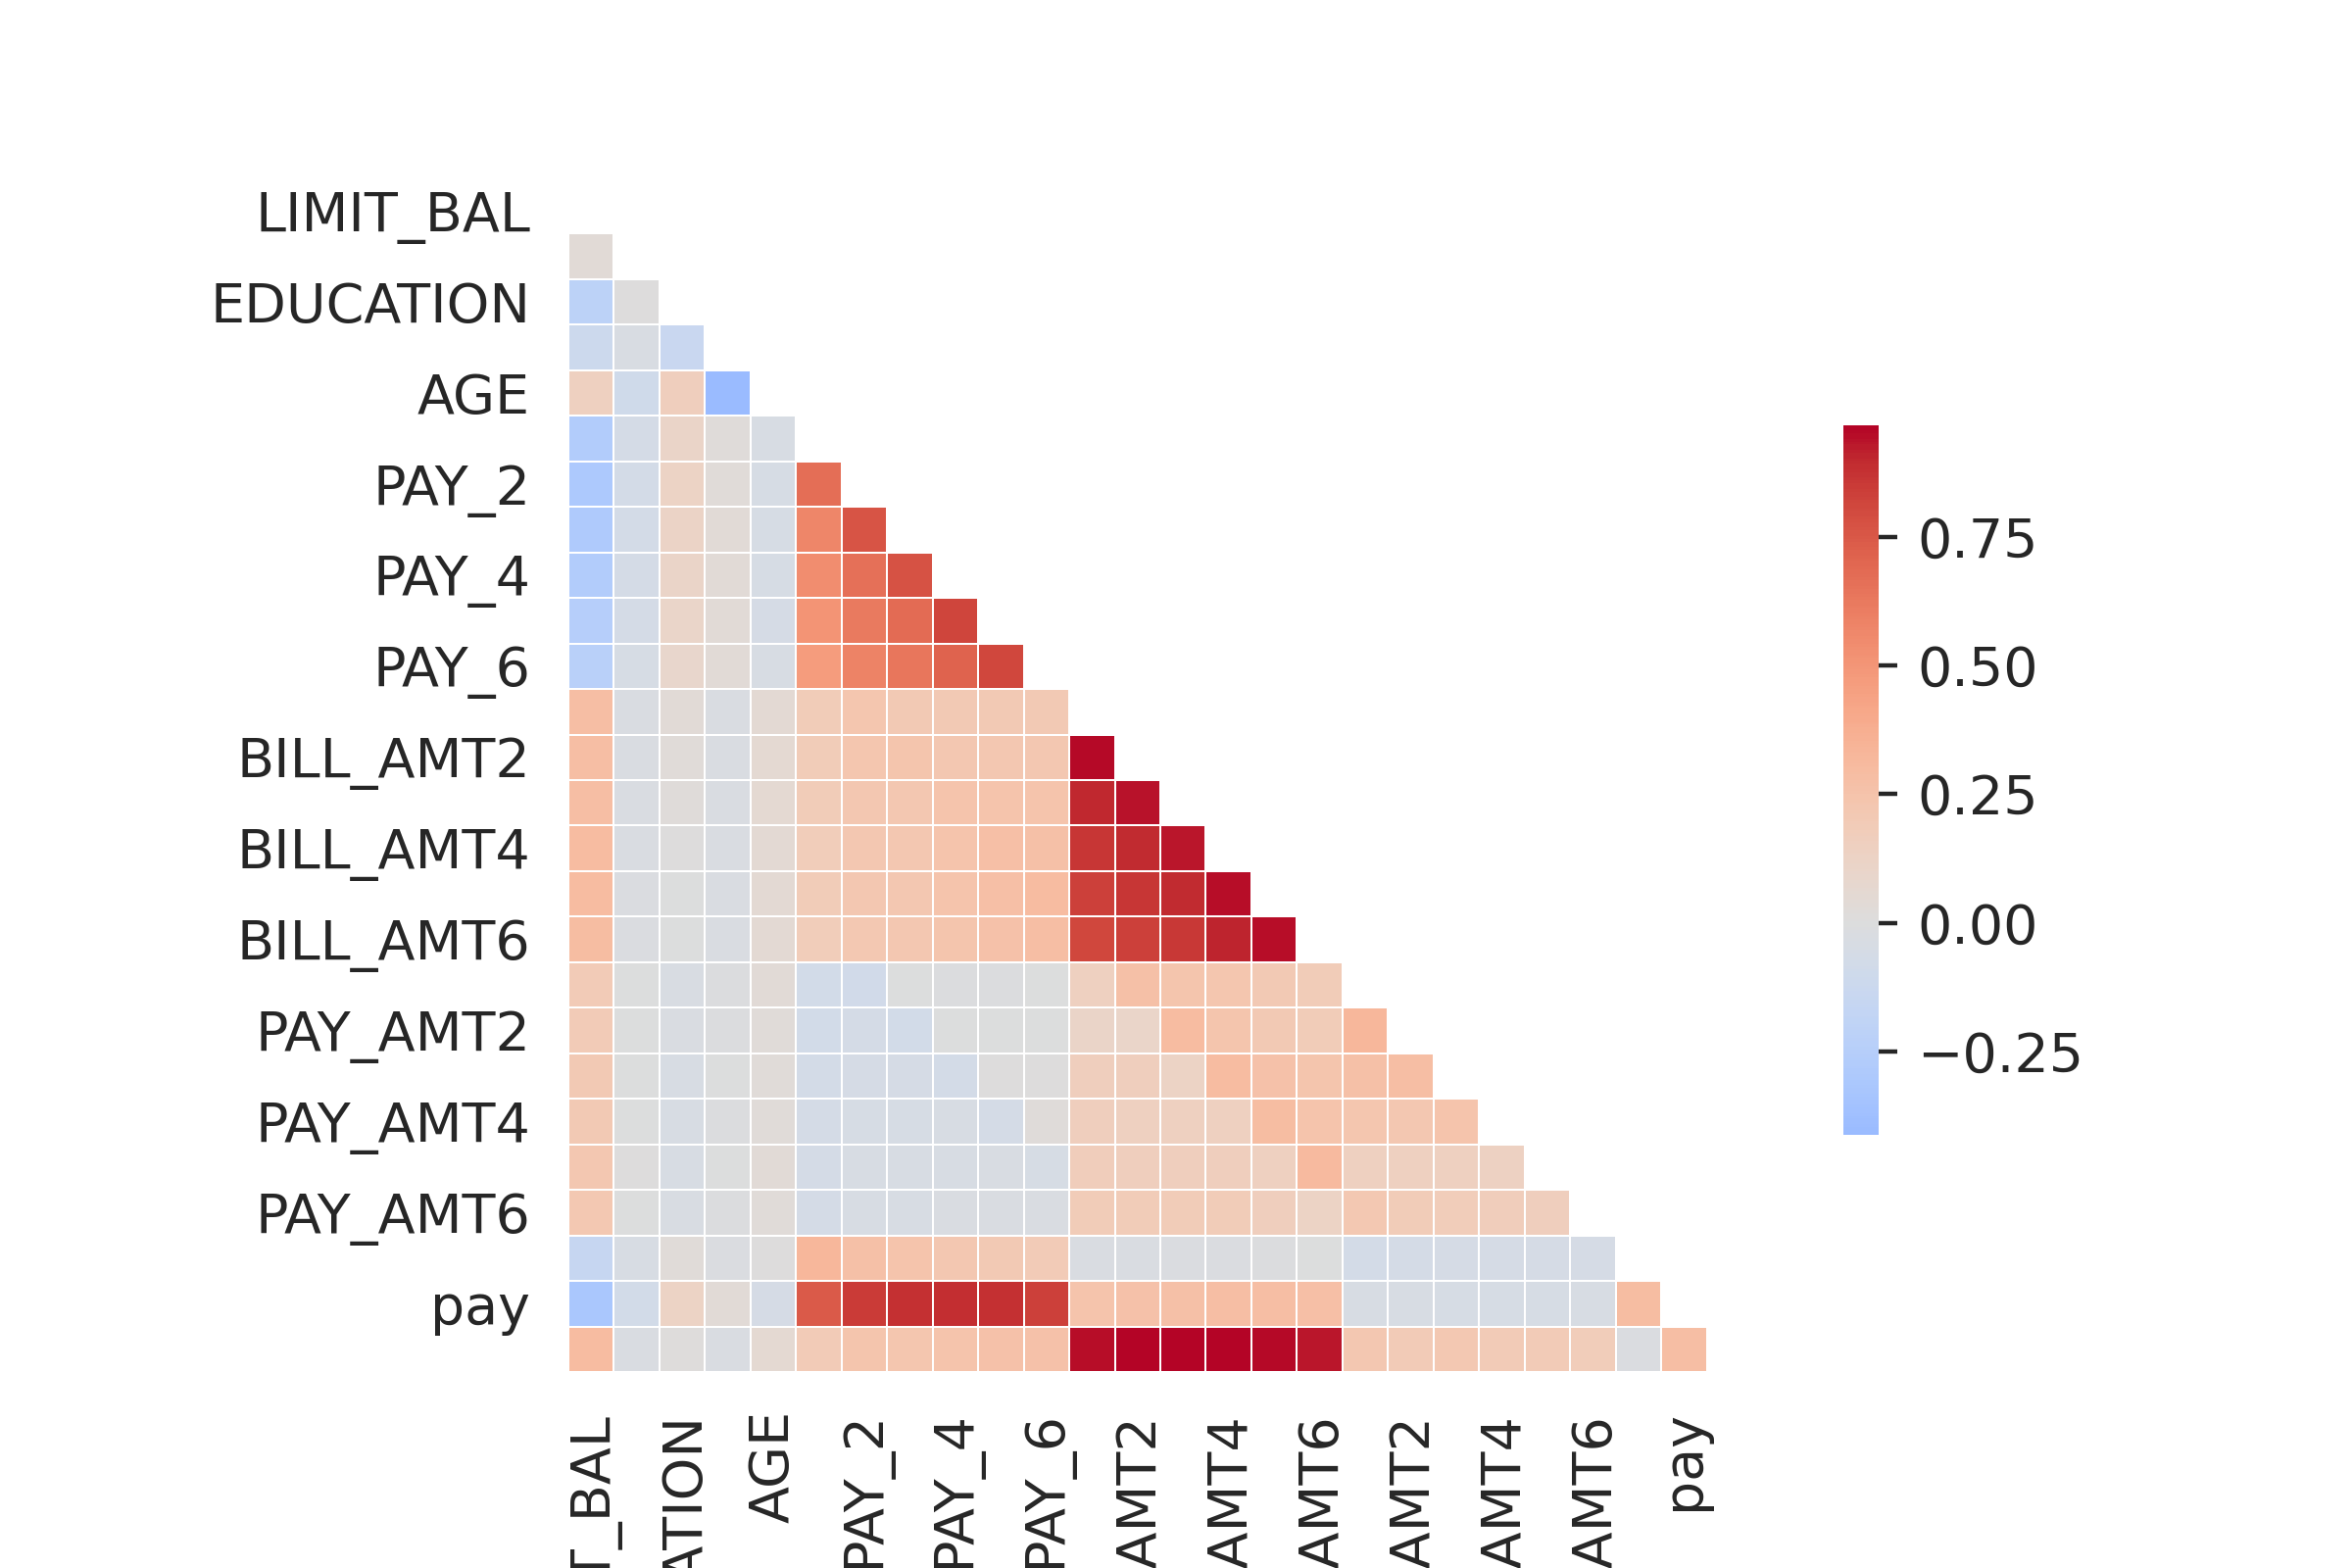
\includegraphics[]{heatmap}
\centering
\caption{Heatmap of correlations}
\label{fig:heatmap}
\end{figure}

\section*{Better understand the features - Setting a baseline score}

At this point the data were directly fitted into a model that required neither feature scaling nor center distribution. The motivation for doing this are, (1)it could be possible to fit a good model with almost no cost of data preparation, (2) to set a baseline score, and most important (3) The models applied are good to understand feature importance.

\subsection*{Score}

The F1 score was set to evaluate the model for two reasons: (1) It is a well-balanced score that assesses accuracy and memory equally, and since we are interested in a well-balanced model, it is naturally a good indicator. (2) Since the dataset is unbalanced, accuracy is no longer a good measure of adequacy.

\subsection*{Models}

Bellow \ref{table:4} is presented the code snippet for the model definition. Cross-validation was applied in combination with GridSearch to set the best model possible and avoid overfitting.

\begin{lstlisting}
rndf_clf = RandomForestClassifier(random_state=42, n_jobs=-1)
extt_clf = ExtraTreesClassifier(random_state=42, n_jobs=-1)  

params = {
    'n_estimators': [200, 300, 400, 500],
    'max_features': ['auto', 'sqrt', 'log2', None],
    'max_leaf_nodes': [10, 15, None]
}

estimators = {}
for estimator in [rndf_clf, extt_clf]:
    estimators[estimator.__class__.__name__] =
     RandomizedSearchCV(estimator=estimator, 
     param_distributions=params, 
     n_jobs=-1, n_iter=15, cv=5, return_train_score=True,
     random_state=42, scoring='f1').fit(X_train, np.ravel(y_train))
                                                                    
\end{lstlisting}

\begin{table}[h!]
\centering
\begin{tabular}{l c }
\toprule
\textbf{Estimator} & \textbf{F1} \\
\midrule
RandomForestClassifier & 0.4779\\
ExtraTreesClassifier & 0.4859\\
\bottomrule
\end{tabular}
\caption{F1}
\label{table:4}
\end{table}

\subsection*{Feature Importance}

Both models suggested that the two most important feature was \textit{History of payment in the previous month}. Besides that, \textit{Credit Limit} and \textit{Age}, are also important. Finally, Features with high correlation between than has a stable scale of importance. 

\section*{Data preparation and Feature Engineering}

The scaling was tackled during the data preparation process that precedes the modeling process. After analyzing the skewness of all numerical variables (Table \ref{table:3}) A log transformation was applied in \textit{Credit Limit}. Finally,
some simulation to reduce colinearity and improve correlations was tried between All variables of history of past payments and between all varibles of Amount of monthly bill, but as no improvement was reached. 

\section*{Model Selection}

Three simple models were selected and a list o paramers were defined. Finally the \textit{GridSearchCV} was used to tune the best estimator for each model selected before. But the result achived was worse than the ensemble methods previous presented. Bellow \ref{table:5} the F1 score for each model:

\begin{table}[h!]
\centering
\begin{tabular}{l c }
\toprule
\textbf{Estimator} & \textbf{F1} \\
\midrule
LinearSVC & 0.3815\\
LogisticRegression & 0.3701\\
KNeighborsClassifier & 0.4256\\
\bottomrule
\end{tabular}
\caption{F1}
\label{table:5}
\end{table}

These selection was also thought because they are very different models and I could use them ensemble. To do so, a \textit{VotingClassifier} was built as follow. However, the ensemble achieve a mean score of 0.3941 and was also rejected.

\begin{lstlisting} 
voting_clf = VotingClassifier(estimators=[
                             ('svm', svm_clf), 
                             ('log', log_clf), 
                             ('knn', knn_clf)], voting='hard')
\end{lstlisting}


\section*{Model Interpretation and Key Findings}

It's clear that the models selected were not able to produce a powerfull model, however, the results are important and have predictive power as well. A hypothetical model that reject all clients would be a very strict model and the F1 of this model would be 0.3623. Therefore, all models trained were better off.

Finally, after six models were tested and different feature engineering were performed, the best fit was: 

\begin{lstlisting} 
ExtraTreesClassifier(random_state=42, n_jobs=-1, 
					 max_features= None, 
					 max_leaf_nodes= 15, 
					 n_estimators= 300)
\end{lstlisting}
\subsection*{Key Findings}

\begin{itemize}
\item Default in the previous month is the most important feature in explaning clients default, Limit credit also has predictive power, but the direction is negative;
\item Education, gender and marriage are less important in explaning default than the history of payments and the credit limit;

\end{itemize}

\subsection*{Test set}

The last phase before presenting the conclusion is that the model were tested against the test dataset and the result is presented below (Table \ref{fig:Confusion Matrix}).

\begin{figure}
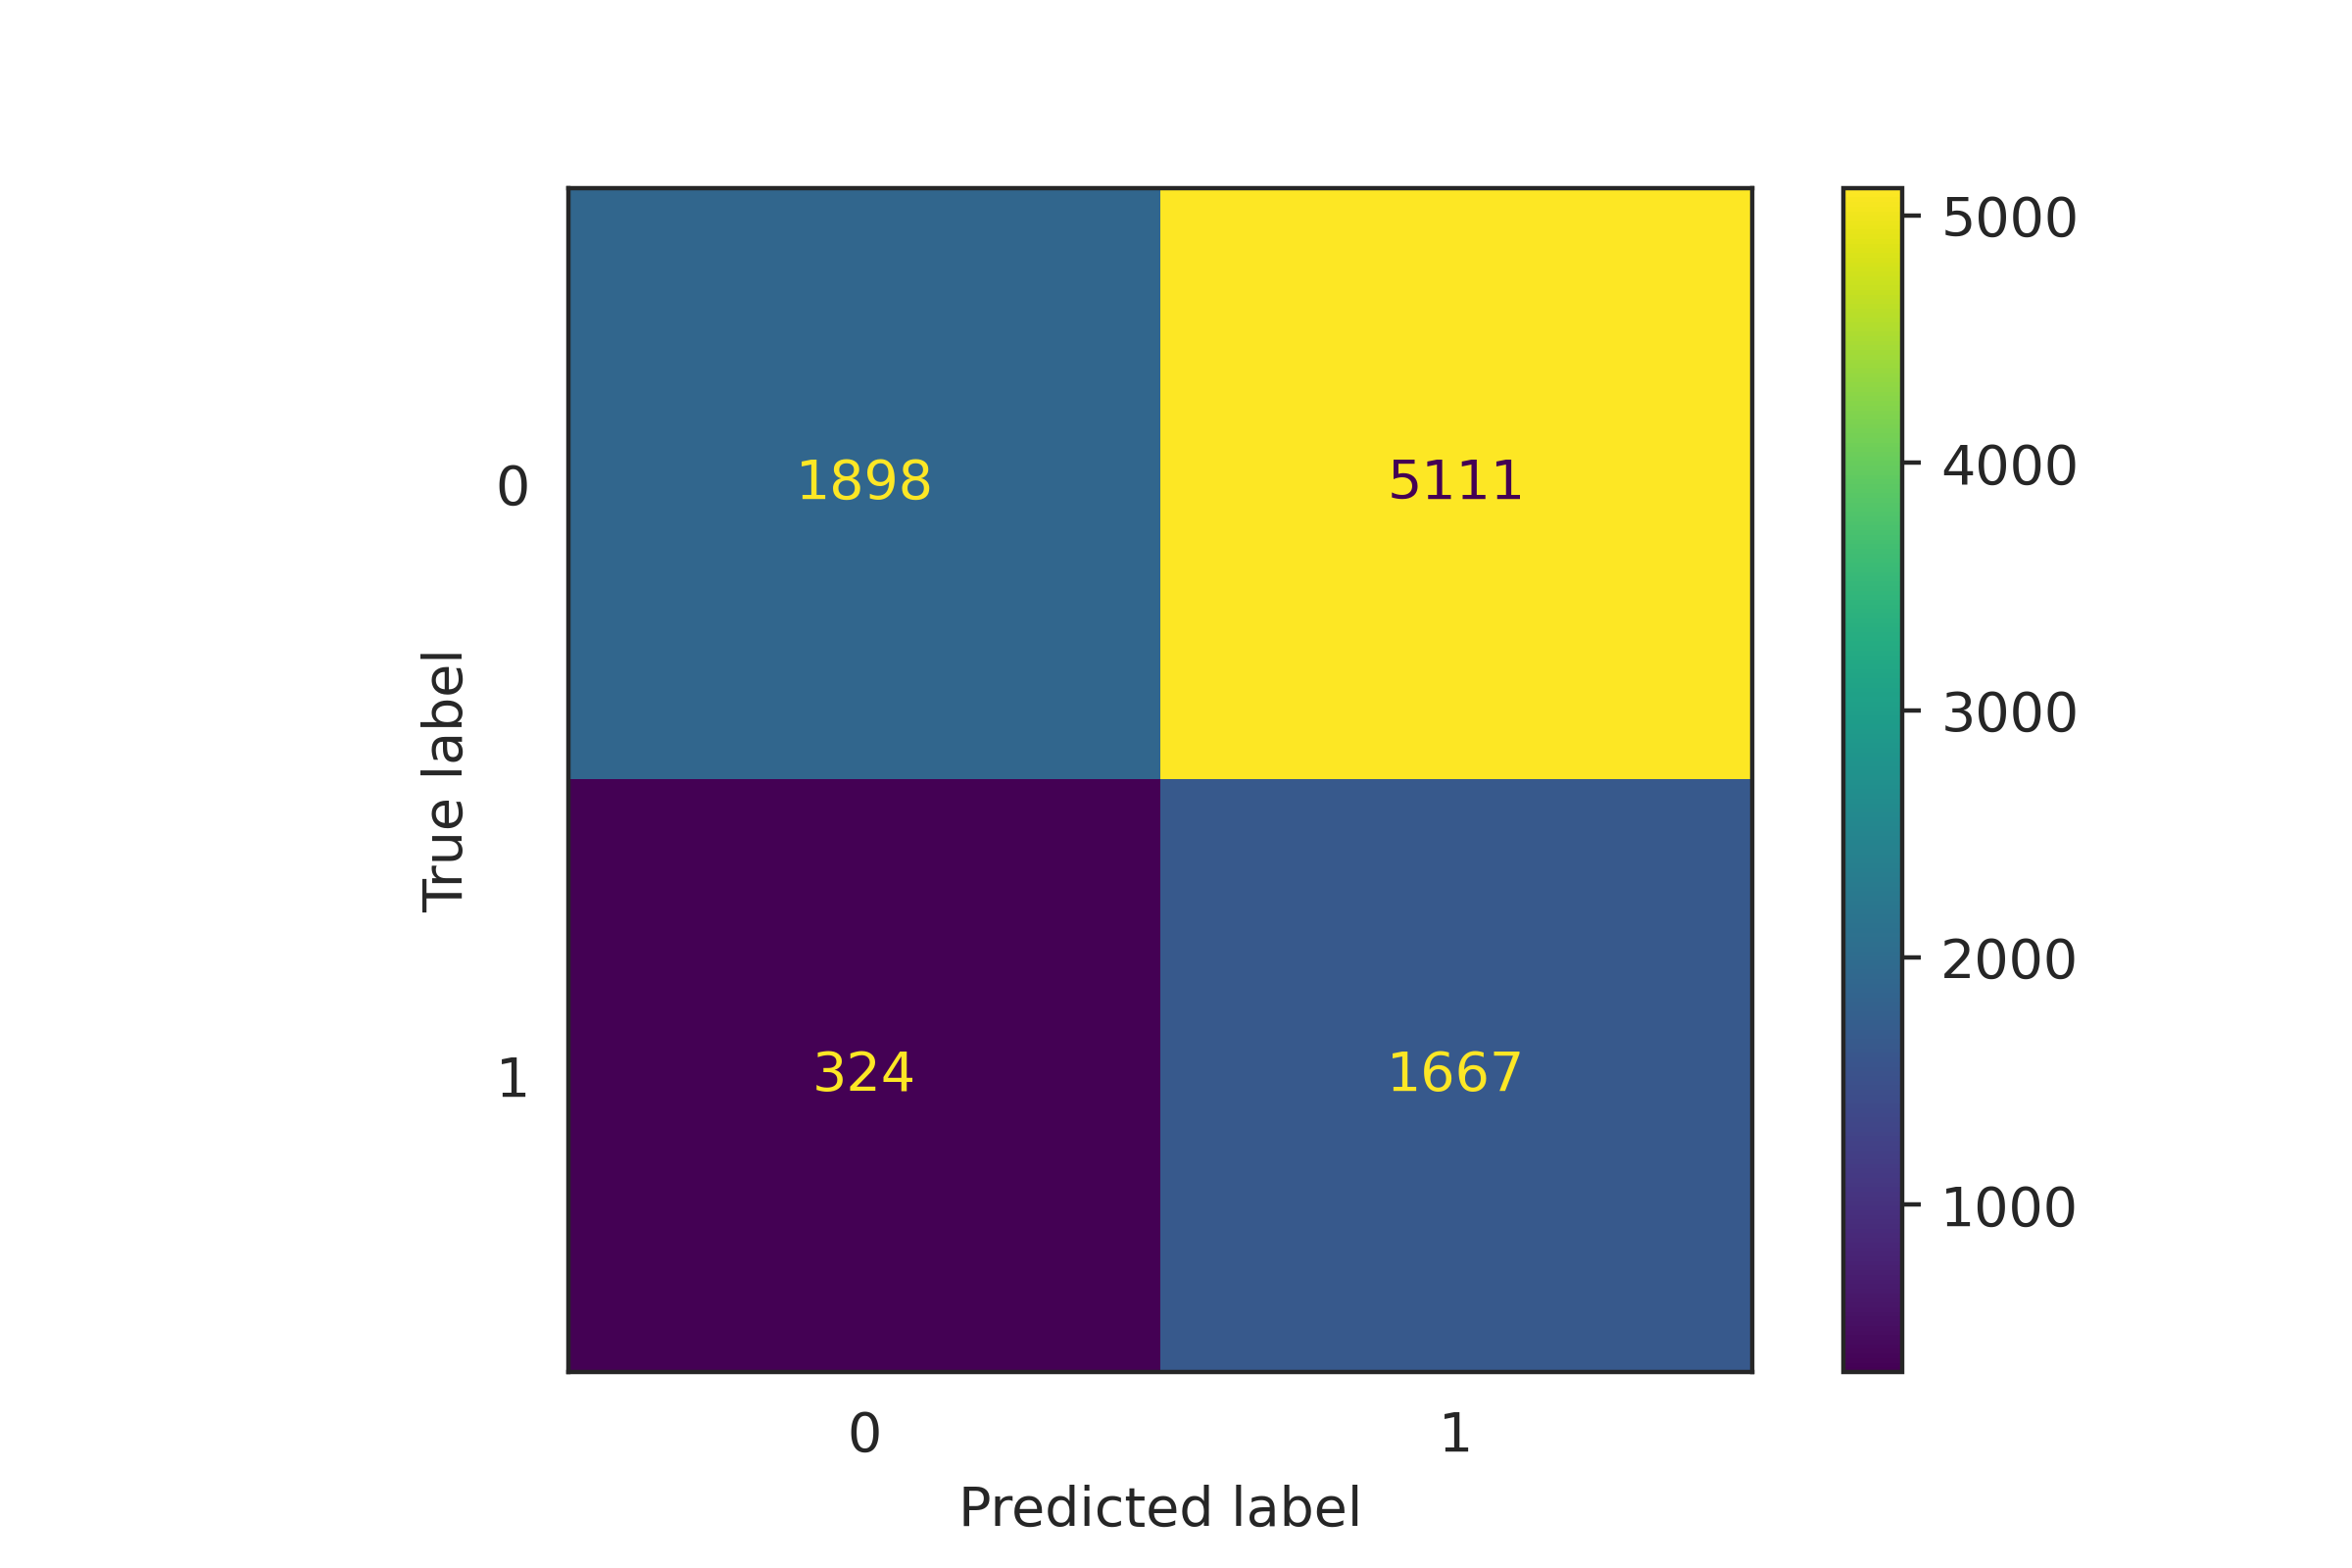
\includegraphics[]{confusion}
\centering
\caption{Confusion Matrix}
\label{fig:Confusion Matrix}
\end{figure}


\section*{Next steps and Improvements}

First of all, there is a field of improvement concerning the dataset analyzed. Definitely more data is required and a robustness can be achieve applying deep learning \cite{Yeh}. Finally, as presented above, credit limit data has explanatory power on credit card defaults, which means that more information related to wealth and employment can improve our predictive power.



\FloatBarrier

\begin{thebibliography}{9}

\bibitem{credit} 
default of credit card clients Data Set,
\\\texttt{https://archive.ics.uci.edu/ml/datasets/default+of+credit+card+clients#}

\bibitem{Yeh}
\\\texttt{Yeh, I. C., & Lien, C. H. (2009). The comparisons of data mining techniques for the predictive accuracy of probability of default of credit card clients. Expert Systems with Applications, 36(2), 2473-2480.}


\end{document}